\documentclass[12pt]{article}
\usepackage{geometry}
\geometry{letterpaper, left=22.5mm, right=22.5mm, top=30mm, bottom=30mm}
\geometry{letterpaper}
\usepackage{amsmath}
\usepackage{amssymb}
\usepackage{enumitem}
\usepackage{fancyhdr}
\usepackage{framed}
\usepackage{tikz}
\usepackage{mathpazo}
%\usepackage{charter}
%\usepackage{newcent}
\usepackage{indentfirst}
\usepackage{booktabs}
\usepackage{graphicx}
\usepackage{float}
\usepackage{makecell}
\usepackage{xcolor}
\usepackage{mdframed}
\usetikzlibrary{trees}
\pagestyle{fancy}
\usepackage{amsthm}
\theoremstyle{definition}
\newtheorem{definition}{Definition}[section]
\theoremstyle{property}
\newtheorem{property}{Property}[section]
\theoremstyle{assumption}
\newtheorem{assumption}{Assumption}[section]
\theoremstyle{example}
\newtheorem{example}{Example}[section]
\theoremstyle{comment}
\newtheorem{comment}{Comment}[section]
\newtheorem{theorem}{Theorem}[section]
\newtheorem{corollary}{Corollary}[theorem]
\newtheorem{lemma}[theorem]{Lemma}
\usepackage{lastpage}
\usepackage{wrapfig}
\usepackage{hyperref}
\usepackage{subcaption}
\usepackage{setspace}
\hypersetup{
colorlinks=true,
linkcolor=black,
filecolor=green, 
urlcolor=blue,
}
\newcommand{\ROM}[1]
    {\MakeUppercase{\romannumeral #1}}
    
    \DeclareMathOperator*{\plim}{plim}
\fancyhead[L]{Econometrics \ROM{2}: Recitation 9}%change each reci
\fancyhead[R]{Spring 2022}
\fancyfoot[C]{\thepage \hspace{1pt} / \pageref{LastPage}}

\fancypagestyle{firstpage}{%
\fancyhf{}%
\renewcommand{\headrulewidth}{0mm}%
  \fancyfoot[C]{\thepage \hspace{1pt} / \pageref{LastPage}}
}
%change title each rec
\title{Introduction to Econometrics \ROM{2}: Recitation 9}

\begin{document}
\linespread{1.25}
\onehalfspacing

\author{Seung-hun Lee\footnote{Contact me at \href{mailto:sl4436@columbia.edu}{sl4436@columbia.edu} if you spot any errors or have suggestions on improving this note.}}
\date{April 4th, 2022}
\maketitle
\thispagestyle{firstpage}

%%%%%%%%%%%%%%%%%%



\section{Nonparametric Regression Models}
\subsection{Asymptotics of the kernel density estimators}
Here is what is known about whether the kernel density estimators are CAN or not, based on Cameron \& Trivedi (2005). Kernel estimator achieves pointwise consistency, or consistent at particular point $y=y_0$ if both the bias and the variance disappear at that point. This is achieved when $h\to0$ and $nh\to\infty$. There is a stronger result which states that $\hat{f}_n(y)$ is consistent at all values of $y$. This requires that $\hat{f}_n(y)$ uniformly converges to $f(y)$. This occurs if $\sup_y |\hat{f}_n(y)-f(y)|\xrightarrow{p}0$. This occurs when $\frac{nh}{\log{n}}\to\infty$, which implies larger $h$ than pointwise consistency.   \par
As for asymptotic normality, we can invoke a central limit theorem to show that they hold. We know the following
\begin{itemize}
\item $E[\hat{f}_n(y)]=f(y)+\frac{1}{2}h^2(f''(y))\int_{-\infty}^\infty u^2K(u)du$
\item $Var(\hat{f}_n(y)) = \frac{1}{nh}f(y) \int_{-\infty}^\infty K^2(u)du$ (the leading term)
\end{itemize}
So to invoke the central limit theorem, we write
\[
\sqrt{nh}\left(\hat{f}_n(y) - f(y) - \frac{1}{2}h^2(f''(y))\int_{-\infty}^\infty u^2K(u)du\right)\sim N\left(0, f(y) \int_{-\infty}^\infty K^2(u)du\right)
\]
As you notice, this is very different from the typical central limit theorem you have observed before. First difference is the effective sample size $nh$. If $h$ is chosen optimally, it is now in the order $O(n^{4/5})$, not $O(n)$ as before. Another is the existence of the bias term. In current settings, the bias and the standard estimates move in the same rate $n^{-2/5}$. Before, the bias converged to 0 quicker than the standard errors so it was ignored. Lastly, there are additional restrictions. We want $f$ to be a $C^2$ function - twice continuously differentiable. This is required for the existence of $f''(y)$. Another condition is a constant  $\int_{-\infty}^\infty u^2K(u)du$ to pin the value of bias.\par
The above result also implies that the (pointwise) confidence interval is defined slightly unconventionally. We define a 95\% pointwise confidence interval at particular $y$ value as
\small{\[
CI = \left[\hat{f}_n(y)-b(y)-1.96\sqrt{\frac{1}{nh}\hat{f}_n(y) \int_{-\infty}^\infty K^2(u)du},\ \hat{f}_n(y)-b(y)+1.96\sqrt{\frac{1}{nh}\hat{f}_n(y) \int_{-\infty}^\infty K^2(u)du}\right]
\]}\normalsize
where $b(y)=\hat{f}_n(y)-\frac{1}{2}h^2(f''(y))\int_{-\infty}^\infty u^2K(u)du$. The complication of the confidence interval comes from the fact that $b(y)$ term cannot be erased. The problem is also complicated further due to the existence of $f''(y)$.  So as an alternative, confidence bands are computed for $f(y)$ over all possible values of $y$, which results in a wider confidence intervals than the pointwise ones. 
\subsection{Estimating a CDF with kernel density estimation}
So far, we have estimated a density - or a pdf - using a kernel density estimator
\[
\hat{f}_n(y) = \frac{1}{nh}\sum_{i=1}^nK\left(\frac{y-y_i}{h}\right)
\]
To get the estimate for the CDF $F(y)$, a natural way of doing this is to use the integrated kernels $\mathcal{K}(y)=\int_{-\infty}^yK(u)du$. Then, we can use
\[
\widehat{F}_n(y) = \frac{1}{n}\sum_{i=1}^n \mathcal{K}\left(\frac{y-y_i}{h}\right)
\]
This sort of estimation is actually nice in the following sense: It fits very well with the kernel estimation $K(\cdot)$ by design, is smooth, and is consistent with $\sqrt{n}$ rate when $n\to\infty, h\to0$. Moreover, it is a better choice than the empirical CDF since there is a significantly less risk of encountering Dirac masses. 

 \subsection{Curse of Dimensionality}
 Now assume that $y$ is not necessarily a scalar, but of dimension $d$. Then we can use a $d$-dimensional kernel $K$ and estimate $f(y)$ with
 \[
 \hat{f}_n(y)= \frac{1}{nh^d}\sum_{i=1}^nK\left(\frac{y-y_i}{h}\right)
 \]
 where $K$ can be a $d$-product of a uni-dimensional kernels. In addition, we are not necessarily confined to using a same bandwith for all $d$ kernels. For instance, if you know that the variance of $y_1$ is larger than $y_2$ you may want higher $h_1$ relative to $h_2$ to avoid variance of the kernel density estimator for the first covariate from being too large. We may want to sphericize if the kernel estimators are correlated. \par
 A bigger concern has to do with the computation cost from using a large $d$. This is what \textbf{curse of dimensionality} refers to. If we return to calculating $E[\hat{f}_n(x)^2]$ term in the variance component of AMISE, (just the leading term)
 
 \footnotesize{\begin{align*}
 E[\hat{f}_n(y)^2]&=E\left[\frac{1}{n^2h^{2d}}\left(\sum_{i=1}^nK\left(\frac{y-y_i}{h}\right)\right)^2\right]\\
 &=E\left[\frac{1}{n^2h^{2d}}\left(\sum_{i=1}^nK^2\left(\frac{y-y_i}{h}\right)+2\sum_{i<j} K\left(\frac{y-y_i}{h}\right)K\left(\frac{y-y_j}{h}\right)\right)\right]\\
 &=\frac{1}{nh^{2d}}\int_{-\infty}^\infty K^2\left(\frac{y-t}{h}\right)f(t)dt+\frac{n(n-1)}{n^2h^{2d}}\left(\int_{-\infty}^\infty K\left(\frac{y-t}{h}\right)f(t)dt\right)^2
 \end{align*}}\normalsize
The leading term is
 \[
\frac{1}{nh^{2d}}\int_{-\infty}^\infty K^2\left(\frac{y-t}{h}\right)f(t)dt \simeq \frac{1}{nh^d}\int K^2(-u)f(y)du
 \]
 since $u$ is actually $d$-dimensional. Thus, the variance is now $O\left(\frac{1}{nh^d}\right)$. Bias remains at the same degree because, 
 \begin{align*}
  E[\hat{f}_n(y)]&=E\left[ \frac{1}{nh^d}\sum_{i=1}^nK\left(\frac{y-y_i}{h}\right) \right]\\
  &=\frac{1}{h^d}\int_{-\infty}^\infty K\left(\frac{y-t}{h}\right)f(t)dt\\
    &=\int_{-\infty}^\infty K(-u)f(y+uh)du \ (\because\text{$u=\frac{t-y}{h}$ and $K(\cdot)$ is an $d$-dimensional multi-kernel})
 \end{align*}
 the rest of the procedure is identical to the univariate kernel estimation case. So bias is still $\frac{1}{2}\int_{-\infty}^\infty K(u)h^2u^2f''(y)du$. \par
  What this means is that $AMISE=Ah^4+\frac{B}{nh^d}$ and the optimal $h$ is solved as
 \[
 h=\left(\frac{Bd}{4An}\right)^{1/(4+d)}
 \]
 Thus, $h$ will be in $n^{-\frac{1}{4+d}}$, bias and standard errors are in $n^{-\frac{2}{4+d}}$ - at an even slower rate that when $d=1$, which was already slower than parametric convergence rate. AMISE would be in order $n^{-\frac{4}{4+d}}$\par
What does this mean for implementation? Loosely speaking, the number of observations required to achieve the same degree of precision as in the lower-dimensional kernels rises. Or more rigorously, the sparseness problem becomes bigger with larger dimensions - fewer observations around $y$ receive substantial weight (or an empty space phenomenon). Silverman documents that the required sample size to accurately estimate density of a standard normal at $0$ rises drastically - 4 for univariate to 842,000 in 10-dimensional. For this reason, tit is rare to use many covariates in nonparametric regressions. \par
 
 One use of multiple kernel estimation is in obtaining the kernel density estimates for the conditional pdf $f(y|x)$. Getting this is not that difficult in principle: We have to obtain the kernel density estimates for the joint pdf $f(y,x)$ with bandwidths $h_y, h_x$ and marginal pdf $f(x)$ with bandwidth $h_x'$. Supppose the dimensions of $x$ and $y$  are $d_x, d_y$. At the end, we get:
 \[
 \hat{f}_n(y|x)= \frac{\hat{f}_n(y,x)}{\hat{f}_n(x)}=\frac{\frac{1}{n(h_x)^{d_x}(h_y)^{d_y}}\sum_{i=1}^n K\left(\frac{y-y_i}{h_y}\right)K\left(\frac{x-x_i}{h_x}\right)}{\frac{1}{n(h_x')^{d_x}}\sum_{i=1}^nK\left(\frac{x-x_i}{h_x}\right)}
 \]
 While obtaining this is relatively easy, it is also easy to where this can go very wrong. If we are working with a large-dimensional data, the asymptotics and the inference becomes difficult because estimators here converge very slowly. The curse of dimensionality plays a huge role here. 
 
  \subsection{Nonparametric Regression: Local polynomial regressions}
 Given the data $(y_i,x_i)$, we are attempting to capture $E[g(y,x)|x]=m(x)$ for some $g(y,x)$. For instance, we can attempt to estimate the conditional expectation by letting $g(y,x)=y$. Note that the conditional expected value can be written as
 \begin{align*}
 E[y|x]&=\int y f_{Y|X}(y|x)dy \\
 &=\int y \frac{f_{Y,X}(y,x)}{f_{X}(x)}dy\\
 &=\frac{\int yf_{Y,X}(y,x)dy}{\int f_{Y,X}(y,x)dy} \ (\because f_X(x) = \int f_{Y,X}(y,x)dy)
 \end{align*}
 We can obtain the nonparametric estimator for the conditional expected value by replacing $f_{Y,X}$ with its kernel estimator. For simplicity, I will assume that the dimension of both $y$ and $x$ is 1 and that the bandwidths are equal. The numerator becomes
 \footnotesize{\begin{align*}
 \int y \hat{f}(y,x)dy&=\int y \frac{1}{nh^2}\sum_{i=1}^n K\left(\frac{x-x_i}{h}\right)K\left(\frac{y-y_i}{h}\right)dy\\
 &= \frac{1}{nh^2}\sum_{i=1}^n K\left(\frac{x-x_i}{h}\right)\int yK\left(\frac{y-y_i}{h}\right)dy\\
 &=\frac{1}{nh^2}\sum_{i=1}^n K\left(\frac{x-x_i}{h}\right)\int (y_i+sh)K\left(s\right)hds \ \left(\because s=\frac{y-y_i}{h}\right)\\
 &= \frac{1}{nh}\sum_{i=1}^n K\left(\frac{x-x_i}{h}\right)y_i\ (\because \int K(s)ds=1, \int sK(s)ds=0)
 \end{align*}}\normalsize
 The denominator can be written as $ \frac{1}{nh}\sum_{i=1}^n K\left(\frac{x-x_i}{h}\right)$. This is because
 \small{\[
 \begin{aligned}
 \int \hat{f}_{Y,X}(y,x)dy&=\int \frac{1}{nh^2}\sum_{i=1}^nK\left(\frac{x-x_i}{h}\right)K\left(\frac{y-y_i}{h}\right)dy\\
 &=\frac{1}{nh^2}\sum_{i=1}^nK\left(\frac{x-x_i}{h}\right)\int K\left(\frac{y-y_i}{h}\right)dy\\
  &=\frac{1}{nh^2}\sum_{i=1}^nK\left(\frac{x-x_i}{h}\right)\int K\left(s\right)hds\\
    &=\frac{1}{nh}\sum_{i=1}^nK\left(\frac{x-x_i}{h}\right) \\
\end{aligned}
 \]}\normalsize
 Thus, the estimator for the conditional expectation becomes
 \[
\hat{m}(x)= \frac{\sum_{i=1}^n y_iK\left(\frac{x-x_i}{h}\right)}{\sum_{i=1}^n K\left(\frac{x-x_i}{h}\right)}
 \]
 Effectively we are putting weight $\frac{K\left(\frac{x-x_i}{h}\right)}{\sum_{i=1}^nK\left(\frac{x-x_i}{h}\right)}$ on each observation $y_i$. This is called a \textbf{local constant estimation} or \textbf{Nadaraya-Watson estimator} in the sense that when we assume that $y_i = a+e_i$ for some constant $a$ , weigh each observation by its kernel density $K\left(\frac{x-x_i}{h}\right)$ and solve the following minimization problem
 \[
 \hat{f}(x)=\arg\min_a\frac{1}{nh}\sum_{i=1}^n(y_i-a)^2K\left(\frac{x-x_i}{h}\right)
 \]
 The first order condition on $a$ yields the following results
 \[
 \sum_{i=1}^ny_iK\left(\frac{x-x_i}{h}\right)=a\sum_{i=1}^nK\left(\frac{x-x_i}{h}\right) \implies a= \frac{\sum_{i=1}^n y_iK\left(\frac{x-x_i}{h}\right)}{\sum_{i=1}^n K\left(\frac{x-x_i}{h}\right)}
 \]\par
 
 As for the asymptotic distribution, We have a similar problem that we did for the kernel density estimation.  Note that
 \[
 y_i = m(x_i)+e_i = m(x) + (m(x_i)-m(x))+e_i
 \]
where $m(x_i)=E[y|x_i]$ is twice continuously differentiable, $f(x)$ is a pdf that is once continuously differentiable, and we assume $E[e_i|x_i]=0, E[e_i^2|x_i=x]=\sigma^2(x)<\infty$. We can express the numerator of $\hat{m}(x)$ as 
\[\begin{aligned}
\frac{1}{nh}\sum_{i=1}^n y_iK\left(\frac{x-x_i}{h}\right) &=\frac{1}{nh}\sum_{i=1}^n K\left(\frac{x-x_i}{h}\right) (m(x) + (m(x_i)-m(x) )+ e_i)\\ 
&=\hat{f}(x)m(x) + \hat{m}_1(x)+\hat{m}_2(x)
\end{aligned}\]
thus, $\hat{m}(x)=\frac{\hat{f}(x)m(x) + \hat{m}_1(x)+\hat{m}_2(x)}{\hat f(x)}= m(x)+\frac{\hat{m}_1(x)}{\hat{f}(x)}+\frac{\hat{m}_2(x)}{\hat{f}(x)}$. So the bias and variance will  be derived from analyzing the last two terms. 
\par
For bias, we need to know $E[\hat{m}_1(x)]$ and  $E[\hat{m}_2(x)]$. Since $E[e_i|x_i]=0$, then $E[e_ih(x_i)]=0$ for any function $h(\cdot)$. So $E\left[e_iK\left(\frac{x-x_i}{h}\right) \right]=0$ and $E[\hat{m}_2(x)]=0$. For $E[\hat{m}_1(x)]$, we work with
\footnotesize{\[\begin{aligned}
E[\hat{m}_1(x)]&=E\left[ \frac{1}{nh}\sum_{i=1}^n K\left(\frac{x_i-x}{h}\right) (m(x_i)-m(x))\right] \ (\because \text{symmetry of } K(\cdot))\\
&= \frac{1}{h}\int K\left(\frac{s-x}{h}\right) (m(s)-m(x))f(s)ds \\
&= \int K\left(u\right) (m(x+hu)-m(x))f(x+hu)du \ \left(\because u=\frac{s-x}{h}\right)\\
&= \int K\left(u\right) (uh m'(x)+ \frac{1}{2}u^2h^2 m''(x)) (f(x)+uhf'(x))du \ \left(\because \text{two Taylor expansions!}\right)\\
&=\int h^2m'(x)f'(x) u^2 K\left(u\right)du +\int \frac{h^2}{2} m''(x)f(x) u^2K(u)du + .... \\
\end{aligned}\]}\normalsize
where ... includes higher order terms than $h^2$ which goes to 0 quicker that $h^2$. We have also used symmetry of the kernel to justify $\int u K(u)du=0$ and so on. If we have $\hat{f}(x)$ that is a consistent density estimator for $f(x)$, we can now write
\[
E[\hat{m}(x)]=m(x) + \int h^2\frac{m'(x)f'(x)}{f(x)} u^2 K\left(u\right)du +\int \frac{h^2}{2} m''(x)u^2K(u)du
\]
Therefore, the bias is still of order $h^2$, but the exact expression becomes
\[
E[\hat{m}(x)]-m(x) = h^2 \left( \frac{m'(x)f'(x)}{f(x)} + \frac{m''(x)}{2} \right)\int u^2K(u)du
\]
\par
As for variance we have
\footnotesize{\[\begin{aligned}
var(\hat{m}_2(x))&=E\left[\left(\frac{1}{nh}\sum_{i=1}^n K\left(\frac{x_i-x}{h}\right)e_i \right)^2\right]\\
&=\frac{1}{nh^2}E\left[\left(K\left(\frac{x_i-x}{h}\right)e_i \right)^2\right] \ (\because IID)\\
&=\frac{1}{nh^2}E\left[\left(K\left(\frac{x_i-x}{h}\right)\sigma(x_i) \right)^2\right] \ (\because \text{condition on }x)\\
&=\frac{1}{nh^2}\int K\left(\frac{s-x}{h}\right)^2\sigma^2(s)f(s)ds \\
&=\frac{1}{nh}\int K\left(u\right)^2\sigma^2(x+hu)f(x+hu)du \simeq\frac{1}{nh}\int K\left(u\right)^2\sigma^2(x)f(x)du
\end{aligned}\]}\normalsize
As for $var(\hat{m}_1(x))$, it is actually $O\left(\frac{h^2}{nh}\right)$ a smaller order than $O\left(\frac{1}{nh}\right)$, so we can worry less about this. Thus, variance is
\[
\frac{1}{nh}\int K\left(u\right)^2\sigma^2(x)f(x)du / f^2(x) = \frac{1}{nh}\frac{\sigma^2(x)}{f(x)}\int K\left(u\right)^2du 
\]
As a result, the asymptotic distribution of the local constant estimator is
\[
\sqrt{nh}\left(\hat{m}(x)-m(x)-h^2 \left( \frac{m'(x)f'(x)}{f(x)} + \frac{m''(x)}{2} \right)\int u^2K(u)du\right)\sim N\left(0, \frac{\sigma^2(x)}{f(x)}\int K\left(u\right)^2du \right)
\]
which is more complicated than the kernel density estimator version. Now we need to worry about the derivatives for the two types of functions. 
\par
Generally, local constant estimators become inaccurate as $f(x)$ is small or at the boundary value in that interpolation becomes less accurate at the ends. Also, as we have seen, the choice of the bandwidth $h$ is trickier. Moreover, the estimate also becomes volatile with $\sigma^2(x)$ - the variance of the $Y$ conditional on $X$. 
\par
 \textbf{Local linear estimation} is an improvement over this. This is when we regress $g(y,x)$ on a constant ($a$) and a linear term ($b(x-x_i)$). In mathematical expression, we solve
 \[
 \min_{a,b}\frac{1}{nh}\sum_{i=1}^n(Y_i-a-b(x-x_i))^2K\left(\frac{x-x_i}{h}\right)
 \]
 and obtain that $\hat{a}=\hat{g}$ and $\hat{b}$ is an estimate of $\frac{\partial g(x)}{\partial x}$. If it happens that the true functional form is linear, then this estimate does not produce a bias. In addition, local linear estimation performs better than local constant estimation in the boundaries of the support for $X$. It also has nicer expression for the asymptotic distribution. While derivation is complicated, the end result is simpler because unlike in local constant estimator, we have explicitly modeled the linear term by controlling for $x-x_i$, and coefficient on this will estimate $m'(x)$. To see why, use the Taylor expansion to check that
$ y_i = m(x_i)+e_i \simeq m(x) + m'(x)(x_i-x)+e_i$. The end result for the asymptotic distribution of local linear estimator is 
 \[
 \sqrt{nh}\left(\hat{m}(x)-m(x)-h^2 \frac{m''(x)}{2} \int u^2K(u)du\right)\sim N\left(0, \frac{\sigma^2(x)}{f(x)}\int K\left(u\right)^2du \right)
 \]
 \par
 Local linear estimator is an improvement since we have simpler form for bias and it behaves better at the areas where $f(x)$ is low or $x$ is at the end of the support for $f(x)$ since it interpolates better than local constant estimator.
  \par
 We can do even more with \textbf{local polynomial estiation} by regressing $g(y,x)$ on a constant, $x-x_i$, $(x-x_i)^2$ and so on. 
The bandwidth can be obtained through cross-validation methods or other rule of thumb methods such as those in Fan, Gijbels (1996). 
  \subsection{Semi-nonparametrics}
\begin{itemize}
\item Flexible approach: Suppose that we are sure that $f(y)$ can be characterized by $f_{m,\sigma}$ where $m,\sigma$ indexes some properties of the density function $f$. Then, by Weierstrass approximation theorem, we can choose a family of positive functions which increases in complexity $P_\theta^1, P_\theta^2,...$ and maximize over the loglikelihood
\[
\sum_{i=1}^n \log{f_{m,\sigma}(y_i)}P_\theta^M(y_i)
\]
\begin{mdframed}[backgroundcolor=green!5] 
\begin{theorem}[Weierstrass Approximation Theorem]  If $f$ is a continuous real-valued function on $[a,b]$ and if any $\epsilon>0$ is given, then there exists a polynomial $P$ on $[a,b]$ s.t. 
\[
|f(x)-P(x)|<\epsilon
\]
for all $x\in[a,b]$
\end{theorem}
\end{mdframed}
\item Mixture of normals: This is a special case of seminonparametrics. Suppose that $Y|X$ is drawn from the two distributions
\begin{itemize}
\item $N_1(m_1(x,\theta), \sigma_1^2(x,\theta))$ with probability $q_1(x,\theta)$
\item $N_2(m_2(x,\theta). \sigma_2^2(x,\theta))$ with probability $q_2(x,\theta)$
\end{itemize}
Then, we apply a maximum likelihood of the following form
\[
\min_\theta \sum_i\sum_k q_k(x_i,\theta)[(y_i-m_k(x_i,\theta))'\sigma_k(x_i,\theta)^{-1}(y_i-m_k(x_i,\theta))+\log\det{\sigma_k(x_i,\theta)}]
\]
As with other MLE estimators, there could be more than one local maxima. Furthermore, the optimal number of $k$ is difficult to determine in practice.
\item Series estimator: Let $\{P_k(x_i)|k=1,2...\}$ be the orthonormal basis for a smooth function. By orthonormal, it means that
\[
\int P_k(x)^2 dx=1, \int P_k(x) P_m(x)=0 \ (k\neq m)
\]
 These could be polynomials of degree $k$, sine functions and so on. What we do here is to run a linear regression that has the following form
\[
y_i = \sum_{k=1}^MP_k(x_i)\theta_k+\epsilon_i
\]
The $\sum_{k=1}^MP_k(x_i)\theta_k$ part is a series approximation to $g(x)$. However, depending on the number of $M$ that we choose, the curse of dimensionality can kick in. 
\item Sieve estimator: It is similar to the series estimator in that it estimates $f(y)$ using the selection of basis $P_k(x_i)$. However, the choice of the basis is data-dependent. Splines or polygonals are the usual choice.
\end{itemize}

\begin{mdframed}[backgroundcolor=yellow!5] 
\begin{example}[Black, Devereux, Lundborg, Majlesi (Restud 2019)]
This paper compares the wealth of the biological and adopted parents to the adopted child to identify whether the inter-generational correlation of wealth is explained by nature or nurture. The figure below plots the within-cohort rank of wealth between children and their parents - biological parents on the left and adoptive parents on the right. The main parametric regression regresses rank of net wealth for children onto rank of wealth for biological and adoptive families and other controls. The parametric results show that the relationship between children's and parental wealth is generally linear, except on the extreme ends of the distribution and that adoptive parents have more deciding role. That finding is verified nonparametrically (epanechnikov kernel with rule-of-thumb bandwidth), where estimation for the children-adoptive parents are steeper and closer to $y=x$ line. 
\begin{figure}[H]
\centering
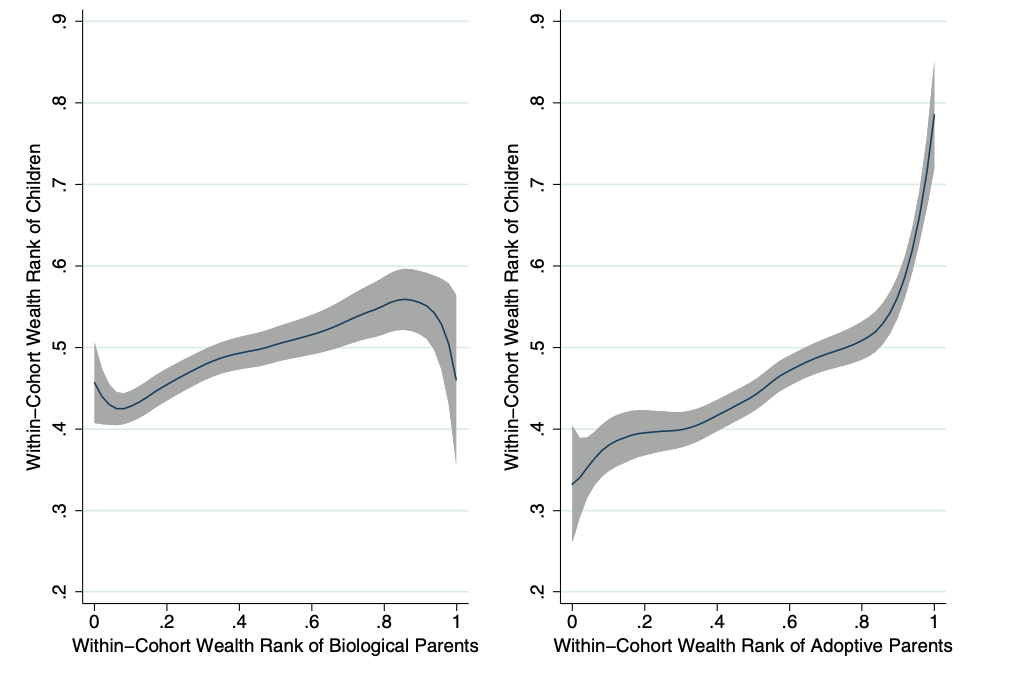
\includegraphics[keepaspectratio, width=0.6\textwidth]{black2.png}
\end{figure}
\end{example}

\begin{example}[Brückner, Ciccone (ECMA 2011)]
The paper shows that democratic change can be triggered by a transitory economic shock. This paper uses variation in rainfall as a source of income shock - negative rainfall shocks induce income shocks for agricultural countries through droughts. Then, the income shock triggers protests and revolutions leading to institutional changes. Authors do verify that in parametric setting, rainfall shock is positively correlated with income and is followed by an improvement in institutions. One of the robustness test done by this paper includes a nonparametric regression of GDP per capita and changes in Polity2 score (higher score indicates more democratic institutions) onto rainfall measures, using local polynomial estimates with epanechikov kernel and bandwidth determined by cross-validation. The results are largely intact but becomes a bit more inaccurate (wider confidence intervals than parametric estimates)
\begin{figure}[H]
\centering
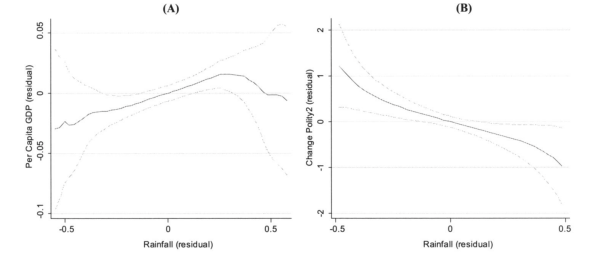
\includegraphics[keepaspectratio, width=0.9\textwidth]{bc_etca.png}
\end{figure}
\end{example}
\end{mdframed}

%%%%%%%%%%%%%%%
\end{document}

